\section{Uniqueness of Integrated Gradients}\label{sec:uniqueness}

Prior literature has relied on empirically evaluating the attribution
technique.  For instance, in the context of an object recognition
task, ~\cite{SBMBM15} suggests that we select the top $k$ pixels by
attribution and randomly vary their intensities and then measure the
drop in score. If the attribution method is good, then the drop in
score should be large. However, the images resulting from pixel
perturbation could be unnatural, and it could be that the scores drop
simply because the network has never seen anything like it in
training.  (This is less of a concern with linear or logistic
models where the simplicity of the model ensures that ablating a
feature does not cause strange interactions.)

\newpage

A different evaluation technique considers images with human-drawn
bounding boxes around objects, and computes the percentage of pixel
attribution inside the box. While for most objects, one would
expect the pixels located on the object to be most important for the
prediction, in some cases the context in which the object occurs may
also contribute to the prediction. The “cabbage butterfly” image from
Figure~\ref{fig:intgrad-finalgrad} is a good example of this where the
pixels on the leaf are also surfaced by the integrated gradients.


Roughly, we found that every empirical evaluation technique we could
think of could not differentiate between artifacts that stem from
perturbing the data, a misbehaving model, and a misbehaving
attribution method.  This was why we turned to an axiomatic approach
in designing a good attribution method (Section~\ref{sec:two-axioms}).
While our method satisfies Sensitivity and Implementation Invariance,
it certainly isn't the unique method to do so.


We now justify the selection of the integrated gradients method in two
steps.  First, we identify a class of methods called Path methods that
generalize integrated gradients.  We discuss that path methods are the
only methods to satisfy certain desirable axioms.  Second, we argue
why integrated gradients is somehow canonical among the different path
methods.

\subsection{Path Methods}
\label{sec:path_methods}

Integrated gradients aggregate the gradients along the
inputs that fall on the straightline between the baseline and
the input. There are many other
(non-straightline) paths that monotonically interpolate between the
two points, and each such path will yield a different attribution method.  For instance,
consider the simple case when the input is two dimensional.
Figure~\ref{fig:three-paths} has examples of three paths, each of which corresponds to a different
attribution method.

\begin{figure}
  \centering
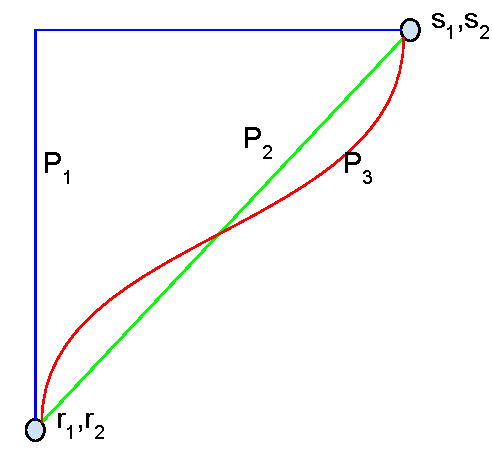
\includegraphics[width=0.5\columnwidth]{./Figures/Paths/integ.pdf}
  \caption{Three paths between an a baseline $(r_1, r_2)$ and an input $(s_1, s_2)$.
    Each path corresponds to a different attribution method. The path $P_2$ corresponds to the path used by integrated gradients.}
  \label{fig:three-paths}
\end{figure}

\newpage
Formally, let $\pathfn = (\pathfn_1, \ldots, \pathfn_n): [0,1]
\rightarrow \reals^n$ be a smooth function specifying a path in
$\reals^n$ from the baseline $\xbase$ to the input $x$, i.e.,
$\pathfn(0) = \xbase$ and $\pathfn(1) = x$.

Given a path function $\pathfn$, \emph{path integrated gradients} are obtained by
integrating the gradients along the path $\pathfn(\sparam)$
for $\sparam \in [0,1]$. Formally, path
integrated gradients along the $i^{th}$ dimension for an input $x$
is defined as follows.
\begin{equation}
\pathintegratedgrads^{\pathfn}_i(x) \synteq \int_{\sparam=0}^{1} \tfrac{\partial F(\pathfn(\sparam))}{\partial \pathfn_i(\sparam)  }~\tfrac{\partial \pathfn_i(\sparam)}{\partial \sparam}  ~d\sparam
\end{equation}
where $\tfrac{\partial F(x)}{\partial x_i}$ is the gradient of
$F$ along the $i^{th}$ dimension at $x$.

Attribution methods based on path integrated gradients are collectively
known as \emph{path methods}. 
Notice that integrated gradients is a path method
for the straightline path specified $\pathfn(\sparam) = \xbase + \sparam\times(x-\xbase)$
for $\sparam \in [0,1]$.

\begin{remark}
  All path methods satisfy Implementation Invariance. This follows from
  the fact that they are defined using the underlying gradients, which
  do not depend on the implementation. They also satisfy Completeness
  (the proof is similar
  to that of Proposition~\ref{prop:additivity})
  and Sensitvity(a) which is implied by Completeness
  (see Remark~\ref{rem:compsens}).
\end{remark}

More interestingly, path methods are the only methods
that satisfy certain desirable axioms. (For formal definitions of the
axioms and proof of Proposition~\ref{prop:path}, see
Friedman~\cite{Friedman}.)

\stitle{Axiom: Sensitivity(b)} (called Dummy in~\cite{Friedman}) If the
function implemented by the deep network does not depend (mathematically)
on some variable, then the attribution to that variable is always
zero.

This is a natural complement to the definition of Sensitivity(a) from
Section~\ref{sec:two-axioms}. This definition captures desired
insensitivity of the attributions.

\stitle{Axiom: Linearity}
Suppose that we linearly composed two deep networks modeled by the
functions $f_1$ and $f_2$ to form a third network that models the
function $a\times f_1 + b\times f_2$, i.e., a linear
combination of the two networks. Then we'd like the attributions for
$a\times f_1 + b\times f_2$ to be the weighted sum of the attributions
for $f_1$ and $f_2$ with weights $a$ and $b$
respectively. Intuitively, we would like the attributions to preserve
any linearity within the network.

  \begin{proposition}(Theorem~1~\cite{Friedman})
    \label{prop:path}
  Path methods are the only
  attribution methods that always satisfy Implementation Invariance,
  Sensitivity(b), Linearity, and Completeness.
\end{proposition}

\begin{remark}
  We note that these path integrated gradients have been used within
  the cost-sharing literature in economics where the function models the
  cost of a project as a function of the
  demands of various participants, and the attributions correspond to
  cost-shares. Integrated gradients correspond to a cost-sharing
  method called Aumann-Shapley~\cite{AS74}.
  Proposition~\ref{prop:path} holds for our attribution problem
  because mathematically the cost-sharing problem corresponds to the
  attribution problem with the benchmark fixed at the zero vector.
  (Implementation Invariance is implicit in the cost-sharing literature
  as the cost functions are considered directly in their mathematical
  form.)
\end{remark}

\subsection{Integrated Gradients is Symmetry-Preserving}

In this section, we formalize why the straightline path chosen by integrated
gradients is canonical.  First, observe that it is the simplest path
that one can define mathematically.  Second, a natural property for
attribution methods is to preserve symmetry, in the following sense.

\stitle{Symmetry-Preserving} Two input variables are symmetric
w.r.t.\ a function if swapping them does not change the function.
For instance, $x$ and $y$ are symmetric w.r.t.\ $F$ if and only if
$F(x, y) = F(y, x)$ for all values of $x$ and $y$.
An attribution method
is symmetry preserving, if for all inputs that have identical values
for symmetric variables and baselines that have identical
values for symmetric variables,  the symmetric variables receive identical
attributions.
%% for all attribution instances,
%% and
%% symmetric w.r.t.\ an attribution instance, if in addition they have
%% the same value at the input in consideration.
%% An attribution method
%% is symmetry preserving, if for all attribution instances, symmetric
%% variables are given identical attributions.

E.g., consider the logistic model $\sigmoid(x_1+x_2+\dots)$.
$x_1$ and $x_2$ are symmetric variables for this model. For
an input where $x_1 = x_2 = 1$ (say) and baseline where $x_1 = x_2 = 0$ (say),
a symmetry preserving method must offer identical attributions to $x_1$ and $x_2$.

It seems natural to ask for symmetry-preserving attribution methods because if two
variables play the exact same role in the network (i.e., they are
symmetric and have the same values in the baseline and the input) then they ought to
receive the same attrbiution.

\begin{theorem}\label{thm:unique}
Integrated gradients is the unique path method that is symmetry-preserving.
\end{theorem}
The proof is provided in Appendix~\ref{sec:proof}.
\begin{remark}
If we allow averaging over the attributions from multiple paths, then
are other methods that satisfy all the axioms in
Theorem~\ref{thm:unique}.
In particular, there is the method by Shapley-Shubik~\cite{ShaShu71}
from the cost sharing literature, and used by~\cite{LundbergL16, DSZ16}
to compute feature attributions (though they were not studying deep networks).
In this method, the attribution is the average of those from $n!$ extremal paths; here $n$
is the number of features. Here each such path considers an ordering
of the input features, and sequentially changes the input feature from
its value at the baseline to its value at the input.
This method yields attributions that are different from integrated gradients. If the function of interest is $min(x_1,x_2)$, the baseline is $x_1=x_2=0$, and the input is $x_1 = 1$, $x_2 =3$,
then integrated gradients attributes the change in the function value entirely to the critical variable $x_1$, whereas Shapley-Shubik assigns attributions of $1/2$ each; it seems somewhat subjective to prefer one result over the other.

We also envision other issues with applying Shapley-Shubik to deep networks:
It is computationally expensive; in an object recognition
network that takes an $100X100$ image as input, $n$ is $10000$, and
$n!$ is a gigantic number.  Even if one samples few paths randomly,
evaluating the attributions for a single path takes $n$ calls to the
deep network. In contrast, integrated gradients is able to operate
with $20$ to $300$ calls. Further, the Shapley-Shubik computation
visit inputs that are combinations of the input and the baseline. It
is possible that some of these combinations are very different from
anything seen during training. We speculate that this could lead to
attribution artifacts.
\end{remark}

\section{Applying Integrated Gradients}
\label{sec:applying}
\stitle{Selecting a Benchmark} A key step in applying integrated
gradients is to select a good baseline. \emph{We recommend that
  developers check that the baseline has a near-zero score}---as
discussed in Section~\ref{sec:method}, this allows us to interpret the
attributions as a function of the input.  But there is more to a good
baseline: For instance, for an object recogntion network it is
possible to create an adversarial example that has a zero score for a
given input label (say elephant), by applying a tiny,
carefully-designed perturbation to an image with a very different
label (say microscope) (cf. ~\cite{adversarial}). The attributions can
then include undesirable artifacts of this adversarially constructed
baseline.  So we would additionally like the baseline to convey a
complete absence of signal, so that the features that are apparent
from the attributions are properties only of the input, and not of the
baseline. For instance, in an object recognition network, a black
image signifies the absence of objects. The black image isn't unique
in this sense---an image consisting of noise has the same
property. However, using black as a baseline may result in cleaner
visualizations of ``edge'' features. For text based networks, we have
found that the all-zero input embedding vector is a good baseline. The
action of training causes unimportant words tend to have small norms,
and so, in the limit, unimportance corresponds to the all-zero
baseline. Notice that the black image corresponds to a valid input to
an object recognition network, and is also intuitively what we humans
would consider absence of signal. In contrast, the all-zero input
vector for a text network does not correspond to a valid input; it
nevertheless works for the mathematical reason described above.


\stitle{Computing Integrated Gradients}
The integral of integrated gradients can be efficiently approximated via a summation. We simply sum the gradients at points occurring at
sufficiently small intervals along the straightline path from
the baseline $\xbase$ to the input $x$.
\begin{equation}
  \begin{split}
    \integratedgrads_i^{approx}(x) \synteq \\
    (x_i-\xbase_i)\times \Sigma_{k=1}^m  \tfrac{\partial F(\xbase + \tfrac{k}{m}\times(x-\xbase)))}{\partial x_i}\times\tfrac{1}{m}
  \end{split}
\end{equation}
Here $m$ is the number of steps in the Riemman approximation of the
integral.  Notice that the approximation simply involves computing the
gradient in a for loop which should be straightforward and efficient
in most deep learning frameworks. For instance, in TensorFlow, it amounts to calling {\tt
  tf.gradients} in a loop over the set of inputs (i.e.,
$\xbase + \tfrac{k}{m}\times(x-\xbase)~\mbox{for}~ k = 1, \ldots, m$), which
could also be batched.
In practice, we find that somewhere between $20$ and $300$ steps are enough to approximate
the integral (within $5\%$); we recommend that developers \emph{check} that the attributions
approximately adds up to the difference beween the score at the input and that at the
baseline (cf. Proposition~\ref{prop:additivity}), and if not increase the step-size $m$.

%% \footnote{Ablation in our setting amounts to zeroing out (or
%%   blacking out) the intensity for the R, G, B channels. We view this
%%   as a natural mechanism for removing the information carried by the
%%   pixel (than, say, randomizing the pixel's intensity as proposed by
%%   ~\cite{SBMBM15}, especially since the black image is a natural baseline
%%   for vision
%%   tasks.}  the top $5000$ pixels ($10\%$ of the image) by importance
%% score, and compute the score drop for the highest scoring object
%% class.  The ablation is performed $100$ pixels at a time, in a
%% sequence of $50$ steps.  At each perturbation step $k$ we measure the
%% average drop in score up to step $k$. This quantity is referred to a
%% \emph{area over the perturbation curve} (AOPC) by~\cite{SBMBM15}.

%% Figure~\ref{fig:aopc} shows the AOPC curve with respect to the number
%% of perturbation steps for integrated gradients and gradients at the
%% image.  AOPC values at each step represent the average over a dataset
%% of $150$ randomly chosen images. It is clear that ablating the top
%% pixels identified by integrated gradients leads to a larger score drop
%% that those identified by gradients at the image.


%% \stitle{Localization}
%% The second evaluation is to consider images with human-drawn bounding
%% boxes around objects, and compute the percentage of pixel attribution
%% inside the bounding box.  We use the 2012 ImageNet object localization
%% challenge dataset to get a set of human-drawn bounding boxes. We run
%% our evaluation on $100$ randomly chosen images satisfying the
%% following properties --- (1) the total size of the bounding box(es) is
%% less than two thirds of the image size, and (2) ablating the bounding
%% box significantly drops the prediction score for the object class. (1)
%% is for ensuring that the boxes are not so large that the bulk of the
%% attribution falls inside them by definition, and (2) is for ensuring
%% that the boxed part of the image is indeed responsible for the
%% prediction score for the image. We find that on $82$ images the
%% integrated gradients technique leads to a higher fraction of the pixel
%% attribution inside the box than gradients at the actual image. The
%% average difference in the percentage pixel attribution inside the box
%% for the two techniques is $8.4\%$.

%% %In light of these findings, we propose using integrated gradients for
%% %object segmentation and localization as a promising future
%% %direction.
%% While these results are promising, we note the following
%% caveat. Integrated gradients are meant to capture pixel importance
%% with respect to the prediction task. 

%% \stitle{Eyeballing}
%% Ultimately, it was hard to come up with a perfect evaluation
%% technique.  So we did spend a large amount of time applying and
%% eyeballing the results of our technique to various networks---the ones
%% presented in this paper, as well as some networks used within
%% products.  For the Inception network, we welcome you to eyeball more
%% visualizations in Figure~\ref{fig:intgrad-finalgrad-more} in
%% the appendix and also at: \url{https://github.com/ankurtaly/Attributions}.
%% While we found our method to beat
%% gradients at the image for the most part, this is clearly a subjective
%% process prone to interpretation and cherry-picking, but is also
%% ultimately the measure of the utility of the approach---debugging
%% inherently involves the human.


%% Object segmentation is an important problem in computer vision that
%% deals with segmenting objects in an image by assigning object class
%% labels to individual pixels in the image. Recent work~\cite{SVZ13, HNH16}
%% has proposed decoupling the object segmentation task from
%% the recognition tasks, and using class-specific saliency maps obtained
%% from a recognition network as an input signal for the
%% segmentation network. In what follows, we focus on how the saliency maps
%% are defined, leaving the specifics of the architecture to the papers
%% referenced above.

%% Prior research has focussed on using gradients of the image for
%% building saliency maps, with the intuition being that pixels located
%% on the object would have significantly higher gradients that pixels in
%% the background. Emperically, we observe that gradients of the actual image
%% suffer from saturation, and fail to distinguish the pixels of the object
%% being recognized (see Figure~\ref{fig:camera-finalgrad}).

%% Instead, we propose using integrated gradients for building saliency
%% maps for object segmentation. From the visualizations in Figure~\ref{fig:intgrad-finalgrad},
%% one can see the pixel attributions resulting from integrated gradients
%% are more localized to the object, and perhaps carry more signal for
%% segmentation; for instance, the emphasize pixels at the object boundary
%% more strongly.

%% In order to objectively evaluate the localization characteristics of
%% integrated gradients, we evaluate them on the 2012 ImageNet object localization
%% challenge dataset. We consider images with human-drawn bounding boxes around
%% objects, and compute the percentage of pixel attribution inside the bounding box.
%% %using
%% %the two techniques.  The technique that results in a larger percentage
%% %is considered better at localizing the object.
%% %
%% We run our evaluation on $100$ randomly chosen images satisfying the
%% following properties --- (1) the total size of the bounding box(es) is
%% less than two thirds of the image size, and (2) ablating the bounding
%% box significantly drops the prediction score for the object class. (1)
%% is for ensuring that the boxes are not so large that the bulk of the
%% attribution falls inside them by definition, and (2) is for ensuring
%% that the boxed part of the image is indeed responsible for the
%% prediction score for the image.

%% We find that on $82$ images the integrated gradients technique leads to
%% a higher fraction of the pixel attribution inside the box than gradients
%% at the actual image. The average difference in the percentage pixel attribution
%% inside the box for the two techniques is $8.4\%$.

%% %In light of these findings, we propose using integrated gradients for
%% %object segmentation and localization as a promising future
%% %direction.
%% While these results are promising, we note the following caveat. Integrated
%% gradients are meant to capture pixel importance with respect to the
%% prediction task. While for most objects, one would expect the pixel
%% located on the object to be most important for the prediction, in some
%% cases the context in which the object occurs may also contribute to
%% the prediction. The “cabbage butterfly” image from Figure~\ref{fig:intgrad-finalgrad}
%% is a good example of this where the pixels on the leaf are also surfaced by the
%% integrated gradients.
